\documentclass[letterpaper,12pt,]{article}

\usepackage[%
    left=1in,%
    right=1in,%
    top=1in,%
    bottom=1.0in,%
    paperheight=11in,%
    paperwidth=8.5in%
]{geometry}%

\usepackage{listings}
\usepackage{graphicx}
\usepackage{amsmath}
\usepackage[font=small,skip=-2pt]{caption}
\usepackage{subcaption}
\usepackage{hyperref}
\usepackage{booktabs}
\usepackage{pdfpages}
\usepackage{pgffor}
\usepackage[section]{placeins}
\lstset{language=[90]Fortran,
  basicstyle=\ttfamily,
  keywordstyle=\color{red},
  commentstyle=\color{green},
  morecomment=[l]{!\ }% Comment only with space after !
}

\lstdefinestyle{mystyle}{
    %backgroundcolor=\color{backcolour},
    %commentstyle=\color{codegreen},
    %keywordstyle=\color{magenta},
    %numberstyle=\tiny\color{codegray},
    %stringstyle=\color{codepurple},
%    basicstyle=\footnotesize,
    basicstyle=\fontsize{7}{9}\selectfont\ttfamily,
    breakatwhitespace=false,
    breaklines=true,
    captionpos=b,
    keepspaces=true,
    numbers=left,
    numberstyle=\footnotesize,
    stepnumber=1,
    numbersep=5pt,
    showspaces=false,
    showstringspaces=false,
    showtabs=false,
    tabsize=2,
    frame=single
}
\lstset{frame=single}

\pagestyle{empty} % Remove page numbering
\linespread{1.5} % Line Spacing

\begin{document}

\begin{titlepage}

\newcommand{\HRule}{\rule{\linewidth}{0.5mm}} % Defines a new command for the horizontal lines, change thickness here

\center % Center everything on the page
 
%----------------------------------------------------------------------------------------
%	HEADING SECTIONS
%----------------------------------------------------------------------------------------


\textsc{\LARGE McGill University}\\[3.5cm]
\textsc{\Large Computational Gasdynamics}\\[0.5cm] 
\textsc{\large MECH 516}\\[2.5cm]

%----------------------------------------------------------------------------------------
%	TITLE SECTION
%----------------------------------------------------------------------------------------

{ \huge \bfseries Project 1}\\[1.5cm] % Title of your document

\HRule \\[0.4cm]
%----------------------------------------------------------------------------------------
%	AUTHOR SECTION
%----------------------------------------------------------------------------------------

\begin{minipage}{0.4\textwidth}
\begin{flushleft} \large
\emph{Name:}\\
Doug \textsc{Shi-Dong} % Your name
\end{flushleft}
\end{minipage}
~
\begin{minipage}{0.4\textwidth}
\begin{flushright} \large
\emph{Student ID:} \\
260466662\\
\end{flushright}
\end{minipage}\\[4cm]

\vfill{}
{\large October 17, 2016}\\[2cm]

\end{titlepage}


\section{Numerical experiments with the linear advection equation}

The first-order Courant, Isaacson, and Rees (CIR) and the Lax-Wendroff schemes are used to solve the linear advection equation.
CIR is first-order accurate in time and space and Lax-Wendroff is second-order accurate in time and space.
The computational domain spans -10 to 240 and the flux at the boundaries use the state variable of the control volume adjacent to the boundary.

\subsection{Exploration of scheme's stability}

The Lax-Wendroff scheme has been chosen to evaluate the solution of the smooth signal problem.
As seen in the previous assignment, the Courant number for which the scheme is stable is lessor equal to 1.
Therefore, the Courant numbers 0.8, 1.02 and 2.0 have been used to demonstrate stability.
It is expected that only the Courant number of 0.8 will be stable.

The first five time steps are shown for different Courant numbers in Fig. \ref{fig:e11}.
Courant numbers of 0.8 and 1.02 seem stable, whereas the Courant number of 2.0 already leads to unstability.
However, if the solution at $t=100$ is required, only the Courant number of 0.8 reaches a valid solution.
The Courant number of 1.02 has velocities of the order 1.0\text{\sc{e}+}18, whereas the Courant number of 2.0 cannot reach $t=100$ without performing an invalid floating point operation.
Plots of the stable solution at time $t=100$ for are provided in Section 1.2.
Plots of the unstable solution are not provided since they are meaningless amplified noise.
\begin{figure}[htb]%
  \centering%
  \begin{subfigure}[b]{\textwidth}
    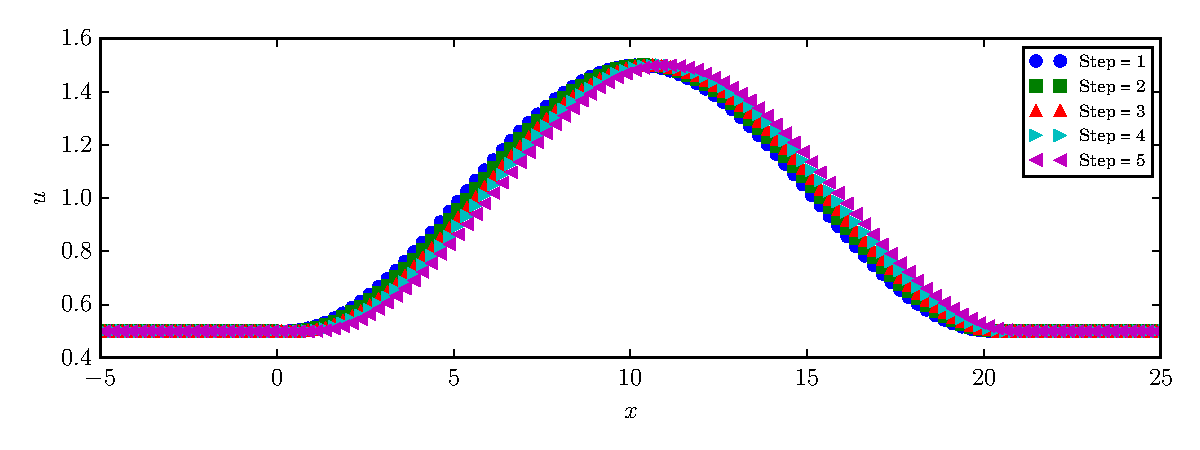
\includegraphics[width = \textwidth,page=1]{figures/exercise11.pdf}
    \caption{CFL = 0.8}
    \label{fig:e11cfl80}
  \end{subfigure}
  \begin{subfigure}[b]{\textwidth}
    \includegraphics[width = \textwidth,page=2]{figures/exercise11.pdf}
    \caption{CFL = 1.02}
    \label{fig:e11cfl102}
  \end{subfigure}
  \begin{subfigure}[b]{\textwidth}
    \includegraphics[width = \textwidth,page=3]{figures/exercise11.pdf}
    \caption{CFL = 2.0}
    \label{fig:e11cfl2}
  \end{subfigure}
\caption{Solution of Lax-Wendroff scheme on smooth signal for different CFL}
\label{fig:e11}
\end{figure}

\subsection{Study of convergence}

Grids with 1000, 2000, and 4000 cells are used for the convergence study, resulting in a spacing of $\Delta 0.25$, $\Delta 0.125$, and $\Delta 0.0625$.

The solution of the triangle-shaped signal is shown in Fig. \ref{fig:e121} for a CFL of 0.8.
The CIR scheme is showing a large amount of numerical dissipation, whereas the Lax-Wendroff scheme is showing a large amount of numerical dispersion.
A the mesh is refined, both schemes retrieve a sharper discontinuity.
Both the CIR and Lax-Wendroff schemes demonstrate less numerical dissipation as the mesh is refined.
However, the Lax-Wendroff scheme exhibits larger oscillations from dispersion, since the mesh refinement results in a sharper discontinuity.
The amount of dispersion is direction related to the change in second-order continuity, so more oscillations are expected with a sharper discontinuity.

\begin{figure}[htb]%
  \centering%
  \begin{subfigure}[b]{0.49\textwidth}
    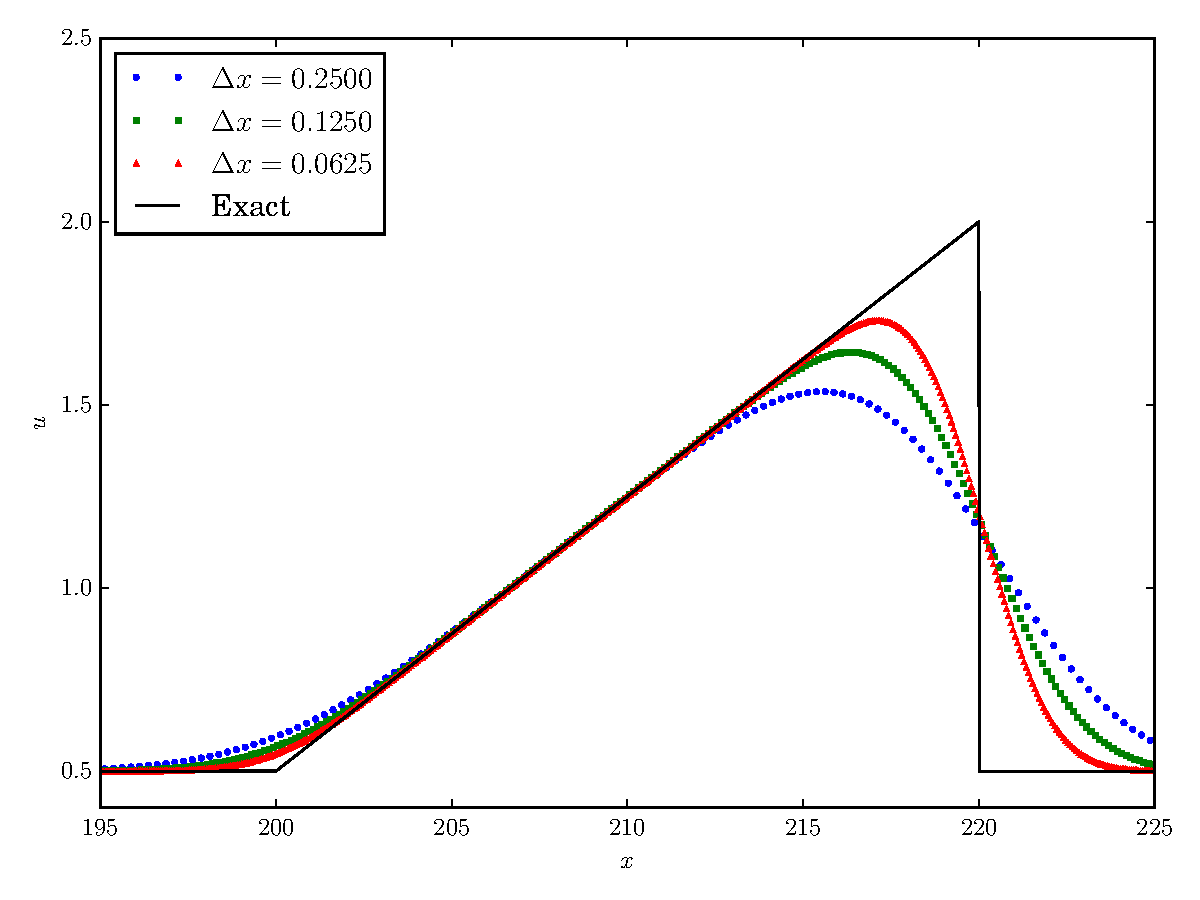
\includegraphics[width = \textwidth,page=1]{figures/exercise12.pdf}
    \caption{CIR}
    \label{fig:cirt}
  \end{subfigure}
  \begin{subfigure}[b]{0.49\textwidth}
    \includegraphics[width = \textwidth,page=2]{figures/exercise12.pdf}
    \caption{Lax-Wendroff}
    \label{fig:lwt}
  \end{subfigure}
\caption{Solution to triangle-shaped-signal with CFL = 0.8 at time $t = 100$}
\label{fig:e121}
\end{figure}

The solution of the smooth signal is shown in Fig. \ref{fig:e122} for a CFL of 0.8.
The same behaviour as previously discussed with dissipation is observed.
A small amount of dispersion can be noticed on the coarsest mesh for the Lax-Wendroff scheme.
However, the smooth solution leads to minimal dispersion.

\begin{figure}[htb]%
  \centering%
  \begin{subfigure}[b]{0.49\textwidth}
    \includegraphics[width = \textwidth,page=3]{figures/exercise12.pdf}
    \caption{CIR}
    \label{fig:cirs}
  \end{subfigure}
  \begin{subfigure}[b]{0.49\textwidth}
    \includegraphics[width = \textwidth,page=4]{figures/exercise12.pdf}
    \caption{Lax-Wendroff}
    \label{fig:lws}
  \end{subfigure}
\caption{Solution to smooth signal with CFL = 0.8 at time $t = 100$}
\label{fig:e122}
\end{figure}

\subsection{Determination of the global order of accuracy}

The actual order of accuracy can be retrieved by taking the slope of the error with respect to the grid size on a log-log plot as shown in Fig. \ref{fig:e13}.
For the triangle signal, the slope of the CIR and Lax-Wendroff schemes are -0.75 and -0.81.
For the smooth signal, the slope of the CIR and Lax-Wendroff schemes are -1.37 and -2.26.
Both scheme demonstrate an order of accuracy lower than first-order on the triangle signal.
This is explained by the presence of a discontinuity where our analysis breaks down due to the inexistence of derivatives.
However, the smooth signal demonstrates first and second order of accuracy as expected.

\begin{figure}[htb]%
  \centering%
  \begin{subfigure}[b]{0.49\textwidth}
    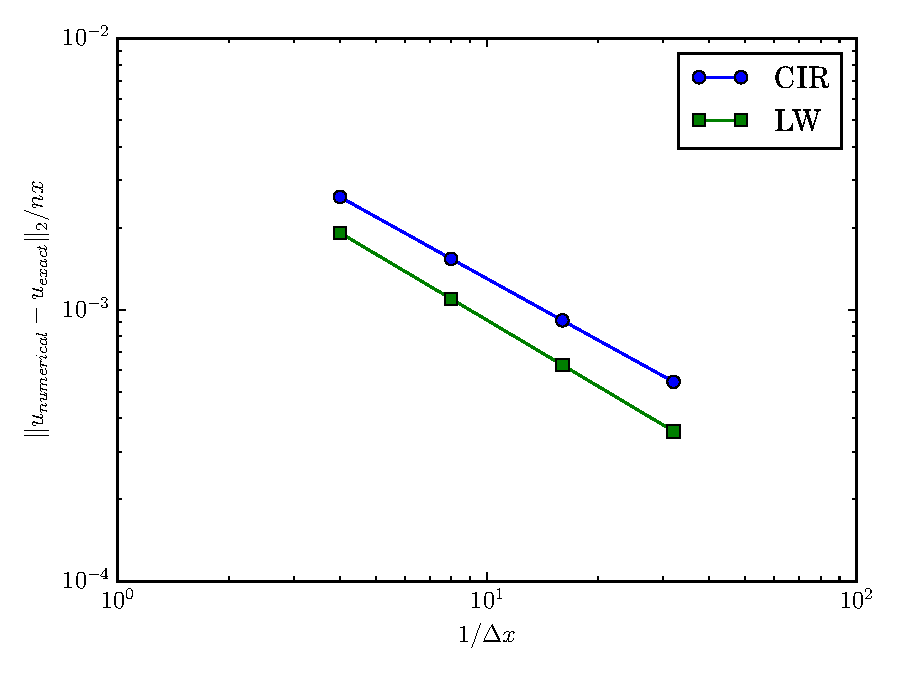
\includegraphics[width = \textwidth,page=1]{figures/exercise13.pdf}
    \caption{Triangle Signal}
    \label{fig:es}
  \end{subfigure}
  \begin{subfigure}[b]{0.49\textwidth}
    \includegraphics[width = \textwidth,page=2]{figures/exercise13.pdf}
    \caption{Smooth Signal}
    \label{fig:et}
  \end{subfigure}
\caption{Order of accuracy}
\label{fig:e13}
\end{figure}


\section*{Results}

The solutions data files have been zipped with the report. They are named p1.dat, p2.dat, and p3.dat for Problem 1, 2 and 3 respectively.

\section*{Code}

Code has been written in FORTRAN available on my Github.
The files have also been zipped with the report.

\url{https://github.com/dougshidong/mech516/tree/master/project1}


\end{document}
